\documentclass[greek]{beamer}
%\usepackage{fontspec}
\usepackage{amsmath,amsthm}
\usepackage{unicode-math}
\usepackage{xltxtra}
\usepackage{graphicx}
\usetheme{CambridgeUS}
\usecolortheme{seagull}
\usepackage{hyperref}
\usepackage{ulem}
\usepackage{xgreek}

\usepackage{pgfpages}
\usepackage{tikz}
\usepackage{tkz-tab}
%\setbeameroption{show notes on second screen}
%\setbeameroption{show only notes}

\usepackage{cancel}

\setsansfont{Noto Serif}

\usepackage{multicol}

\usepackage{appendixnumberbeamer}

\usepackage{polynom}

\usepackage{pgffor}

\setbeamercovered{transparent}
\beamertemplatenavigationsymbolsempty

\title{Κωνικές Τομές}
\subtitle{Έλλειψη}
\author[Λόλας]{Κωνσταντίνος Λόλας}
\date{}

\begin{document}

\begin{frame}
 \titlepage
\end{frame}

\section{Θεωρία}
\begin{frame}{Γεωμετρικοί τόποι παντού}
 Κάναμε
 \begin{enumerate}
  \item<1-> σταθερή απόσταση από ένα σημείο
  \item<2-> ίση απόσταση από δύο σημεία
  \item<3-> σταθερή απόσταση από ευθεία
  \item<4-> ίση απόσταση από δύο ευθείες
  \item<5-> ίση απόσταση από σημείο και ευθεία
 \end{enumerate}
 \only<5> {άρα ψάχοντνας για επόμενο...} \only<6> {\emph{σταθερό άθροισμα αποστάσεων από δύο σημεία?}}
\end{frame}

\begin{frame}{Φύγαμε για Geogebra}
 \href{https://www.geogebra.org/classic/wfmc8s24}{\beamergotobutton{Geogebra}}
\end{frame}

\begin{frame}{Λίγο πιο απλά?}
 Φυσικά. Θα ασχοληθούμε μόνο με τις ελλείψεις που έχουν εστίες πάνω στους άξονες συμμετρικές ως προς την αρχή των αξόνων
\end{frame}

\begin{frame}{Ακόμα πιο απλά?}
 Και πάλι φυσικά.
 \begin{itemize}
  \item Εστίες $Ε(γ,0)$ και $Ε'(-γ,0)$ ή
  \item Εστίες $Ε(0,γ)$ και $Ε'(0,-γ)$
 \end{itemize}
\end{frame}

\begin{frame}[label=Έλλειψη]{Πιο επίσημα?}
 \begin{block}{Εξίσωση Έλλειψης 1}
  Η έλλειψη με εστίες τα σημεία $Ε(γ,0)$, $Ε'(-γ,0)$ και σταθερό άθροισμα $2α$ είναι η
  $$\dfrac{x^2}{α^2}+\dfrac{y^2}{α^2-γ^2}=1$$
 \end{block}
 ή πιο \emph{ωραία}
 \begin{block}{Εξίσωση Έλλειψης}
  Η έλλειψη με εστίες τα σημεία $Ε(γ,0)$, $Ε'(-γ,0)$ και σταθερό άθροισμα $2α$ είναι η
  $$\dfrac{x^2}{α^2}+\dfrac{y^2}{β^2}=1$$
  όπου $β^2=α^2-γ^2$
 \end{block}

 \hyperlink{ΑπόδειξηΕξίσωσης}{\beamerbutton{Πάμε για απόδειξη?}}

\end{frame}

\begin{frame}{Ορισμοί}
 \begin{itemize}
  \item<1-> \emph{Εστιακή απόσταση}: Το μήκος $ΕΕ'=2γ$
  \item<2-> \emph{Κορυφές έλλειψης}: Τα σημεία $Α(α,0)$, $Α'(-α,0)$, $Β(0,β)$ και $Β'(0,-β)$
  \item<3-> \emph{Μεγάλος άξονας}: Το ευθύγραμμο τμήμα $ΑΑ'$ μήκους $2α$
  \item<4-> \emph{Μικρός άξονας}: Το ευθύγραμμο τμήμα $ΒΒ'$ μήκους $2β$
  \item<5-> \emph{Κέντρο}: Το σημείο $(0,0)$
  \item<6-> \emph{Διάμετρος}: Το ευθύγραμμο τμήμα που ορίζουν δύο συμμετρικά ως προς το κέντρο της έλλειψης
  \item<7-> \emph{Εκκεντρότητα}: Ο λόγος $ε=\dfrac{γ}{α}$
  \item<8-> \emph{Όμοιες Ελλείψεις}: Δύο ελλείψεις με ίσες εκκεντρότητες
 \end{itemize}
\end{frame}

\begin{frame}{Τα ίδια, αλλά ανάποδα!}
 Αλλάξτε τα $x$ με τα $y$!
 \begin{block}{Εξίσωση Έλλειψης 2}
  Η έλλειψη με εστίες τα σημεία $Ε(0,γ)$, $Ε'(0,-γ)$ και σταθερό άθροισμα $2α$ είναι η
  $$\dfrac{x^2}{α^2-γ^2}+\dfrac{y^2}{α^2}=1$$
 \end{block}
 ή πιο \emph{ωραία}
 \begin{block}{Εξίσωση Έλλειψης}
  Η έλλειψη με εστίες τα σημεία $Ε(0,γ)$, $Ε'(0,-γ)$ και σταθερό άθροισμα $2α$ είναι η
  $$\dfrac{x^2}{β^2}+\dfrac{y^2}{α^2}=1$$
  όπου $β^2=α^2-γ^2$
 \end{block}
\end{frame}

\begin{frame}{Πρώτες παρατηρήσεις}
 \begin{itemize}
  \item<1-> Οι κορυφές βρίσκονται εύκολα για $x=0$ ή $y=0$
  \item<2-> Η έλλειψη κλείνεται στο ορθογώνιο που έχει πλευρές παράλληλες στους άξονες που διέρχονται από τις κορυφές
  \item<3-> Ο μεγάλος άξονας είναι πάντα ο άξονας των εστιών
  \item<4-> Το κέντρο της έλλειψης είναι κέντρο συμμετρίας
  \item<5-> Οι άξονες είναι άξονες συμμετρίας
  \item<6-> Για την εκκεντρότητα ισχύει $0<ε<1$
  \item<7-> Αν $γ=0$ τότε η έλλειψη μετετρέπεται σε κύκλο
 \end{itemize}
\end{frame}

\begin{frame}[label=Εφαπτόμενη]{Εφαπτομένη έλλειψης}
 \begin{block}{Εξίσωση}
  Η εξίσωση της εφαπτομένης της έλλειψης $\dfrac{x^2}{α^2}+\dfrac{y^2}{β^2}=1$ στο σημείο της $(x_1,y_1)$ είναι η $$\dfrac{xx_1}{α^2}+\dfrac{yy_1}{β^2}=1$$
 \end{block}

 \hyperlink{ΑπόδειξηΕφαπτόμενη}{\beamerbutton{Πάμε για απόδειξη?}}
\end{frame}

\begin{frame}[label=Ιδιότητες]{Ιδιότητα Έλλειψης}
 Η κάθετη στην εφαπτόμενη σε ένα σημείο της έλλειψης $Μ$, διχοτομεί την γωνία $\widehat{ΕΜΕ'}$

 \centering
 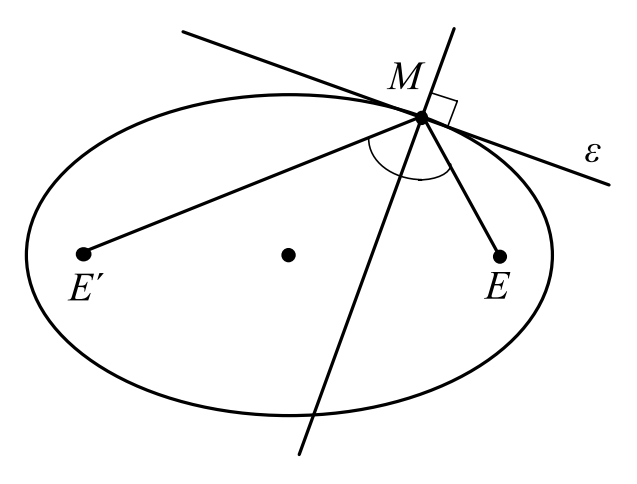
\includegraphics[width=0.5\textwidth]{"../images/reflection2.png"}

 \hyperlink{Απόδειξη}{\beamerbutton{Πάμε για απόδειξη?}}
\end{frame}

\section{Ασκήσεις}
\subsection{Άσκηση 1}
\begin{frame}[label=Άσκηση1,t]{Εξάσκηση 1}
 Έστω η έλλειψη με εστίες $Ε'(-3,0)$, $Ε(3,0)$ και το μήκος του κικρού άξονα είναι $8$
 \begin{enumerate}
  \item<1-> Να βρείτε το μήκος του μεγάλου άξονα
  \item<2-> Να βρείτε την εξίσωσή της
  \item<3-> Να βρείτε την εκκεντρότητά της
 \end{enumerate}

 % \hyperlink{Λύση1}{\beamerbutton{Λύση}}
\end{frame}

\subsection{Άσκηση 2}
\begin{frame}[label=Άσκηση2,t]{Εξάσκηση 2}
 Έστω η έλλειψη που έχει κέντρο την αρχή των αξόνων και εστίες στον άξονα $y'y$. Αν η έλλειψη διέρχεται από το σημείο $Μ\left( 1,\dfrac{10\sqrt{2}}{3} \right) $ και έχει εκκεντρότητα $ε=\dfrac{4}{5}$, να βρείτε
 \begin{enumerate}
  \item<1-> την εξίσωσή της
  \item<2-> τις εστίς και τα μήκη των αξόνων της
 \end{enumerate}

 % \hyperlink{Λύση2}{\beamerbutton{Λύση}}
\end{frame}

\subsection{Άσκηση 3}
\begin{frame}[label=Άσκηση3,t]{Εξάσκηση 3}
 Να βρείτε την εξίσωση της εφαπτομένης της έλλειψης $C:x^2+3y^2=4$, που διέρχεται από το σημείο $Ρ(2,1)$

 % \hyperlink{Λύση3}{\beamerbutton{Λύση}}
\end{frame}

\subsection{Άσκηση 4}
\begin{frame}[label=Άσκηση4,t]{Εξάσκηση 4}
 Δίνεται η έλλειψη $C:2x^2+y^2=6$ και το σημείο της $Μ(μ,2)$, $μ<0$. Να βρείτε την εξίσωση της ευθείας που διχοτομεί την γωνία $\widehat{Ε'ΜΕ}$ όπου $Ε'$ και $Ε$ οι εστίες της $C$

 % \hyperlink{Λύση4}{\beamerbutton{Λύση}}
\end{frame}

\subsection{Άσκηση 5}
\begin{frame}[label=Άσκηση5,t]{Εξάσκηση 5}
 Έστω ότι η ευθεία $ε:y=-8x+2$ εφάπτεται στην έλλειψη $C$ στο σημείο της $Μ(2,1)$. Να βρείτε την εξίσωση της έλλειψης $C$ που έχει κέντρο την αρχή των αξόνων

 % \hyperlink{Λύση5}{\beamerbutton{Λύση}}
\end{frame}

\subsection{Άσκηση 6}
\begin{frame}[label=Άσκηση6,t]{Εξάσκηση 6}
 Δίνεται η έλλειψη $C:3x^2+4y^2=16$. Να δείξετε ότι η ευθεία $ε:3x+2y-8=0$ εφάπτεται στην έλλειψη $C$ και να βρείτε το σημείο επαφής.

 % \hyperlink{Λύση6}{\beamerbutton{Λύση}}
\end{frame}

\subsection{Άσκηση 7}
\begin{frame}[label=Άσκηση7,t]{Εξάσκηση 7}
 Δίνεται η έλλειψη $C:\dfrac{x^2}{5}+\dfrac{y^2}{4}=1$. Από το σημείο $Ρ(2,-3)$ φέρουμε τις εφαπτόμενες $ΡΑ$, $ΡΒ$ προς την $C$. Να βρείτε την απόσταση του σημείου $Ρ$ από την ευθεία $ΑΒ$

 %\hyperlink{Λύση7}{\beamerbutton{Λύση}}
\end{frame}

\subsection{Άσκηση 8}
\begin{frame}[label=Άσκηση8,t]{Εξάσκηση 8}
 Να βρείτε τις κοινές εφαπτόμενες του κύκλου $C_1:x^2+y^2=2$ και της έλλειψης $C_2:x^2+3y^2=3$

 %\hyperlink{Λύση8}{\beamerbutton{Λύση}}
\end{frame}

\subsection{Άσκηση 9}
\begin{frame}[label=Άσκηση9,t]{Εξάσκηση 9}
 Έστω τα σημεία $Ε'(-4,0)$ και $Ε(4,0)$. Να βρείτε το γεωμετρικό τόπο των σημείων $Μ$, για τα οποία ισχύει
 $$|ΜΕ|+|ΜΕ'|=10$$
 και στη συνέχεια την εξίσωσή του

 %\hyperlink{Λύση9}{\beamerbutton{Λύση}}
\end{frame}

\subsection{Άσκηση 10}
\begin{frame}[label=Άσκηση10,t]{Εξάσκηση 10}
  Να βρείτε το γεωμετρικό τόπο των σημείων $Μ$, για τα οποία ισχύει
  $$3\overrightarrow{OM}^2+2\overrightarrow{OM}\cdot \overrightarrow{OM'}=5$$
  όπου $M'$ το συμμετρικό σημείο του $M$ ως προς τον άξονα $x'x$

  %\hyperlink{Λύση10}{\beamerbutton{Λύση}}
\end{frame}

\subsection{Άσκηση 11}
\begin{frame}[label=Άσκηση11,t]{Εξάσκηση 11}
  Αν $Μ$ σημείο της έλλειψης $C:\dfrac{x^2}{5}+\dfrac{y^2}{4}=1$, με εστίες τα σημεία $Ε'$ και $Ε$, να δείξετε ότι
  $$|\overrightarrow{ΜΕ'}|\cdot |\overrightarrow{ΜΕ}|+\overrightarrow{ΟΜ}^2=9$$
  όπου $Ο$ η αρχή των αξόνων

  %\hyperlink{Λύση11}{\beamerbutton{Λύση}}
\end{frame}

\subsection{Άσκηση 12}
\begin{frame}[label=Άσκηση12,t]{Εξάσκηση 12}
  Να βρείτε την εξίσωση της χορδής $ΑΒ$ της έλλειψης $C:4x^2+9y^2=36$, που έχει μέσο το σημείο $Μ(2,1)$

  %\hyperlink{Λύση12}{\beamerbutton{Λύση}}
\end{frame}

\subsection{Άσκηση 13}
\begin{frame}[label=Άσκηση13,t]{Εξάσκηση 13}
  Δίνεται η έλλειψη $C_1:x^2+4y^2=4$ και ο κύκλος $C_2:x^2+y^2-10x+24=0$. Να βρείτε την ελάχιστη και την μέγιστη απόσταση ενός σημείου της $C_1$ από ένα σημείο της $C_2$

  %\hyperlink{Λύση13}{\beamerbutton{Λύση}}
\end{frame}

\subsection{Άσκηση 14}
\begin{frame}[label=Άσκηση14,t]{Εξάσκηση 14}
  Να βρείτε το πλησιέστερο σημείο της έλλειψης $C:x^2+2y^2=6$ από την ευθεία $x+y-8=0$

  %\hyperlink{Λύση14}{\beamerbutton{Λύση}}
\end{frame}

\appendix

\section{}
\begin{frame}
 Στο moodle θα βρείτε τις ασκήσεις που πρέπει να κάνετε, όπως και αυτή τη παρουσίαση
\end{frame}

\section{Αποδείξεις}
\begin{frame}[label=ΑπόδειξηΕξίσωσης]{Απόδειξη εξίσωσης έλλειψης}
 Οι εστίες είναι οι $Ε(γ,0)$, $Ε(-γ,0)$ και η σταθερή απόσταση είναι $2α$. Για κάθε σημείο $M(x,y)$ θα ισχύει:
 $$|ME|+|ΜΕ'|=2α$$
 \begin{gather*}
  \sqrt{\left(x-γ\right)^2+(y-0)^2}+\sqrt{\left(x+γ\right)^2+(y-0)^2}=2α \\ \pause
  \sqrt{\left(x-γ\right)^2+y^2}=2α-\sqrt{\left(x+γ\right)^2+y^2} \\ \pause
  \left(   \sqrt{\left(x-γ\right)^2+y^2}\right)^2=\left( 2α-\sqrt{\left(x+γ\right)^2+y^2} \right)^2 \\ \pause
  \only<4>{x^2-2γx+γ^2+y^2=4α^2-4α\sqrt{\left(x+γ\right)^2+y^2}+x^2+2γx+γ^2+y^2 \\} \pause
  \only<1-3,5->{\cancel{x^2}-2γx+\bcancel{γ^2}+\xcancel{y^2}=4α^2-4α\sqrt{\left(x+γ\right)^2+y^2}+\cancel{x^2}+2γx+\bcancel{γ^2}+\xcancel{y^2} \\} \pause
  4α\sqrt{\left(x+γ\right)^2+y^2}=4α^2+4γx
  \cancel{4}α\sqrt{\left(x+γ\right)^2+y^2}=\cancel{4}α^2+\cancel{4}γx
 \end{gather*}
\end{frame}

\begin{frame}{Απόδειξη εξίσωσης έλλειψης}
 Οι εστίες είναι οι $Ε(γ,0)$, $Ε(-γ,0)$ και η σταθερή απόσταση είναι $2α$. Για κάθε σημείο $M(x,y)$ θα ισχύει:
 $$|ME|+|ΜΕ'|=2α$$
 \begin{gather*}
  α\sqrt{\left(x+γ\right)^2+y^2}=α^2+γx \\ \pause
  α^2\left(\left(x+γ\right)^2+y^2\right)=(α^2+γx)^2 \\ \pause
  \only<3>{α^2x^2+2α^2γx+α^2γ^2+α^2y^2=α^4+2α^2γx+γ^2x^2 \\} \pause
  \only<1-2,4->{α^2x^2+\cancel{2α^2γx}+α^2γ^2+α^2y^2=α^4+\cancel{2α^2γx}+γ^2x^2 \\} \pause
  (α^2-γ^2)x^2+α^2y^2=α^4-α^2γ^2 \\ \pause
  (α^2-γ^2)x^2+α^2y^2=α^2(α^2-γ^2) \\ \pause
  \dfrac{x^2}{α^2}+\dfrac{y^2}{α^2-γ^2}=1
 \end{gather*}

 \hyperlink{Έλλειψη}{\beamerbutton{Πίσω στη θεωρία}}
\end{frame}

\begin{frame}[label=ΑπόδειξηΕφαπτόμενη]{Απόδειξη εφαπτόμενης}
 Άντε ρε που θέλετε και την απόδειξη!

 \hyperlink{Εφαπτόμενη}{\beamerbutton{Πίσω στη θεωρία}}
\end{frame}

\begin{frame}[label=Απόδειξη]{Απόδειξη ανακλαστικής ιδιότητας}
 Είπαμε!

 \hyperlink{Ιδιότητες}{\beamerbutton{Πίσω στη θεωρία}}
\end{frame}


% \section{Λύσεις Ασκήσεων}
% \begin{frame}
%  \tableofcontents
% \end{frame}
%
% \subsection{Άσκηση 1}
% \begin{frame}[label=Λύση1]
%  Με θεώρημα ενδιαμέσων τιμών. Η συνάρτηση είναι συνεχής στο $[10,11]$ με $f(10)=1024$ και $f(11)=2048$. Αφού $2023\in (1024,2048)$ υπάρχει $x_0$...
%
%  \hyperlink{Άσκηση1}{\beamerbutton{Πίσω στην άσκηση}}
% \end{frame}
%
% \subsection{Άσκηση 2}
% \begin{frame}[label=Λύση2]
%  Με Bolzano ή με μέγιστης ελάχιστης τιμής και ΘΕΤ.
%
%  \begin{gather*}
%   f(3)<f(2)<f(1) \\
%   3f(3)<f(1)+f(2)+f(3)<3f(1) \\
%   f(3)<\dfrac{f(1)+f(2)+f(3)}{3}<f(1)
%  \end{gather*}
%
%  \hyperlink{Άσκηση2}{\beamerbutton{Πίσω στην άσκηση}}
% \end{frame}
%
% \subsection{Άσκηση 3}
% \begin{frame}[label=Λύση3]
%  Προφανές ελάχιστο στα $x_1=1$ και $x_2=3$. Ως συνεχής στο $[1,3]$ έχει σίγουρα ΚΑΙ μέγιστο στο $(1,3)$
%
%  \hyperlink{Άσκηση3}{\beamerbutton{Πίσω στην άσκηση}}
% \end{frame}
%
% \subsection{Άσκηση 4}
% \begin{frame}[label=Λύση4]
%  Η συνάρτηση `απόστασης` $f(x)-x$ είναι ορισμένη στο κλειστό διάστημα και έχει σίγουρα μέγιστο
%
%  \hyperlink{Άσκηση4}{\beamerbutton{Πίσω στην άσκηση}}
% \end{frame}
%
% \subsection{Άσκηση 5}
% \begin{frame}[label=Λύση5]
%  Όμοια με την Άσκηση 2
%
%  \hyperlink{Άσκηση5}{\beamerbutton{Πίσω στην άσκηση}}
% \end{frame}
%
% \subsection{Άσκηση 6}
% \begin{frame}[label=Λύση6]
%  \begin{enumerate}
%   \item Είναι γνησίως αύξουσα άρα $(f(+\infty),f(-\infty))$
%   \item Προφανώς $[f(0),f(1)]$...
%  \end{enumerate}
%
%  \hyperlink{Άσκηση6}{\beamerbutton{Πίσω στην άσκηση}}
% \end{frame}

\end{document}
